\documentclass[page number]{beamer}
\usetheme[sectionpage=none,numbering=fraction,progressbar=foot]{metropolis}

\usepackage{pgf,tikz}
\usetikzlibrary{arrows}
\usetikzlibrary{positioning,shapes,fit}
\usepackage{xcolor}
\usepackage{amssymb}
\usepackage{amsmath}

\makeatletter
\makeatother

\setcounter{tocdepth}{1} % remove subsection from table of contents

% colors
\definecolor{mDarkRed}{HTML}{6F1616}
\definecolor{mDarkGreen}{HTML}{106235}
\definecolor{mTeal}{HTML}{112233}
\definecolor{mBlack}{HTML}{000000}
\setbeamercolor{normal text}{fg=mTeal}
\setbeamercolor{alerted text}{fg=mDarkRed}
\setbeamercolor{example text}{fg=mDarkGreen}
\setbeamercolor{title separator}{fg=purple,bg=mBlack}

\def\outline{
  \begin{frame}[plain,noframenumbering]
    \frametitle{Outline}
    \tableofcontents[currentsection]
  \end{frame}
}


\begin{document}
\title[The Power of Clause Learning]{Understanding the Power of Clause Learning}

\author{Paul Beame \hfill Henry Kautz \hfill Ashish Sabharwal}
\vfill
\date{
  \vfill
  \textbf{Presentation:}\quad Aur\`ele Barri\`ere
  \vfill
  \textbf{03/10/18}}

\def\outline{
  \begin{frame}[plain,noframenumbering]
    \frametitle{Outline}
    \tableofcontents[currentsection]
  \end{frame}
}

\begin{frame}[plain,noframenumbering]
  \vspace{-2cm}
  \maketitle
  \vspace{-4cm}
\end{frame}

%% \metroset{sectionpage=none}

\metroset{sectionpage=progressbar}

\begin{frame}{Context}
  \begin{block}{Published in IJCAI in 2003}
  \end{block}
  \vfill
  \begin{block}{Motivation}
    \begin{itemize}
    \item Deciding SAT as quickly as possible has many uses.
    \item DPLL-based algorithms work well.
    \item The most efficient algorithms are just variants of DPLL with clause learning.
    \item No formal work to explain the success of clause learning.
    \end{itemize}
  \end{block}
\end{frame}

\begin{frame}{The SAT decision problem}
  \begin{block}{SAT}
    Given a Conjunctive Normal Form (CNF) formula, decide if there exists an assignment that satisfies it. \\
    NP-complete.
  \end{block}
  \vfill
  \begin{exampleblock}{Techniques}
    \begin{itemize}
    \item DPLL and its variants, \textbf{clause learning} and \textbf{restarts}
    \item General Resolution
    \item Regular Resolution
    \item \dots
    \end{itemize}
  \end{exampleblock}
\end{frame}

\begin{frame}{Davis-Putnam-Logemann-Loveland (DPLL)}
  \begin{block}{DPLL algorithm}
    Branch on variables (following a \textbf{branching order}). \\
    Apply \textbf{unit propagation} and \textbf{pure literal} rules.\\
    If a conflict is found, backtrack to the last choice.
  \end{block}
  \vfill
  \begin{exampleblock}{Clause Learning}
    At each conflict, draw a conflict graph then learn a new clause.\\
    Very efficient.
  \end{exampleblock}
  \vfill
  \begin{exampleblock}{Restarts}
    At any point during the execution of the algorithm, forget all your choices and start from the beginning, while keeping the learned clauses.
  \end{exampleblock}
      
\end{frame}

\begin{frame}{Resolution Proof Systems}
  \begin{block}{General Resolution}
    $$(x \vee A) \wedge (\neg x\vee B) \wedge C \quad\sim_{\text{SAT}}\quad (A \vee B) \wedge C$$
    Resolving on $x$. Applying the resolution rule and getting to the empty clause means the formula is unsatisfiable.
  \end{block}
  \vfill
  \begin{alertblock}{General Resolution is not efficiently implementable}
    It's hard to find the good choices for the variables to resolve on.
  \end{alertblock}
  \vfill
  \begin{block}{Regular Resolution Variant}
    Any variable can be resolved upon at most once.\\
    Used in the original DP in 1960.
  \end{block}
\end{frame}

\begin{frame}{Comparing SAT methods for unsatisfiable formulas}
  \begin{block}{Proof Complexity [Cook and Reckhow, 1977]}
    Compare the size of the shortest proof of unsatisfiability.
  \end{block}
  \vfill
  \begin{block}{Size of the Shortest Proof?}
    \begin{itemize}
    \item Resolution systems: number of times we applied the resolution rule.
    \item DPLL-based: number of choices made (including the ones leading to conflicts).
    \end{itemize}
  \end{block}
  \vfill
  \begin{alertblock}{Unsatisfiable Formulas Only}
  \end{alertblock}

\end{frame}

\begin{frame}{Comparing SAT methods for unsatisfiable formulas}
  \begin{exampleblock}{Best-Case Scenario}
    We are not evaluating heuristics, only the technique to prove unsatisfiability.\\
    This framework doesn't account for the difficulty of making the right choices.\\
    This framework doesn't account for the time to apply rules.
  \end{exampleblock}
  \vfill
  \begin{block}{Relevance for satisfiable formulas}
    [Achlioptas, Beame, Molloy, 2001] shows that good complexity results on unsatisfiable formulas imply good results on satisfiable formulas as well.
  \end{block}
    
\end{frame}

\begin{frame}{Known Results}
  \begin{center}
    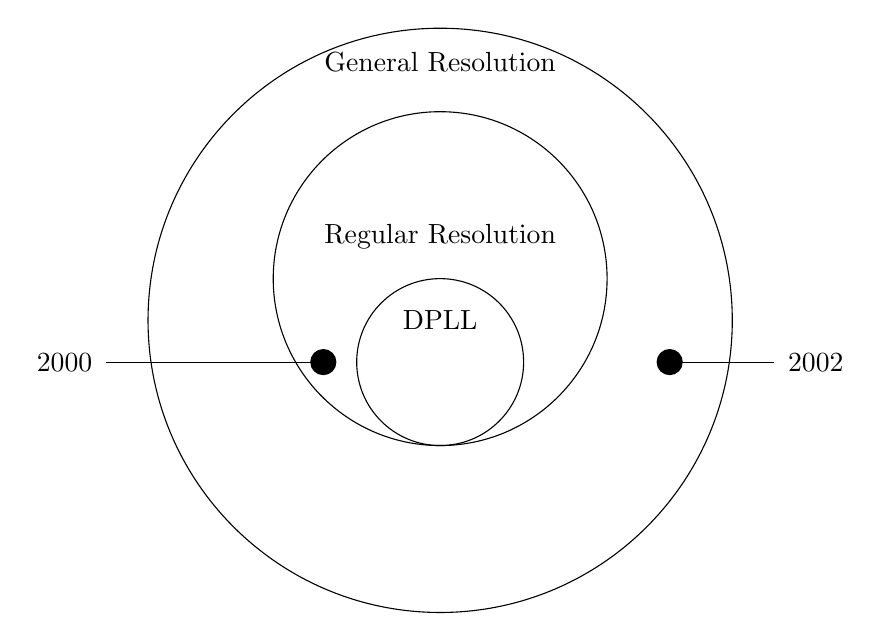
\begin{tikzpicture}[scale=0.53]
      \draw (0,0) circle (2cm);
      \draw (0,2) circle (4cm);
      \draw (0,1) circle (7cm);
      \node[] at (0,1) {DPLL};
      \node[] at (0,3) {Regular Resolution};
      \node[] at (0,7.2) {General Resolution};
      \draw[fill=black] (-2.8,0) circle (0.3cm);
      \draw (-8,0) -- (-2.8,0);
      \node[] at (-9,0) {2000};
      \draw[fill=black] (5.5,0) circle (0.3cm);
      \draw (8,0) --  (5.5,0);
      \node[] at (9,0) {2002};
    \end{tikzpicture}
  \end{center}
\end{frame}
  
\begin{frame}{Contribution}
  \begin{exampleblock}{Contributions}
    \begin{itemize}
    \item The first formal analysis of Clause Learning
    \item A new learning scheme, \textbf{FirstNewCut}
    \item \textbf{DPLL + clause learning} can be better than \textbf{Regular Resolution}
    \item \textbf{DPLL + clause learning + restarts} is equivalent \textbf{to General Resolution}
    \item Experimental Results
    \end{itemize}
  \end{exampleblock}
\end{frame}

\begin{frame}{Known Results}
  \begin{center}
    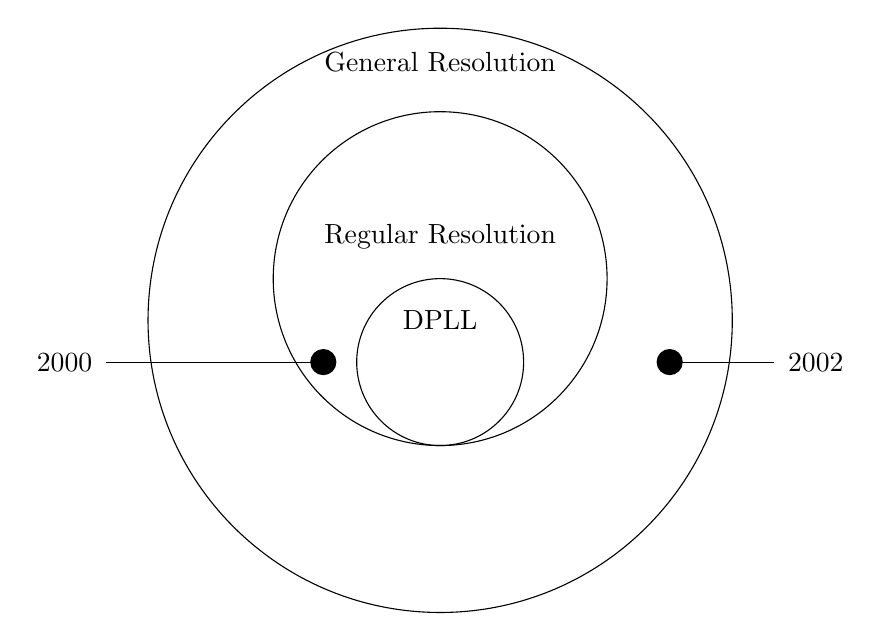
\begin{tikzpicture}[scale=0.53]
      \draw (0,0) circle (2cm);
      \draw (0,2) circle (4cm);
      \draw (0,1) circle (7cm);
      \node[] at (0,1) {DPLL};
      \node[] at (0,3) {Regular Resolution};
      \node[] at (0,7.2) {General Resolution};
      \draw[fill=black] (-2.8,0) circle (0.3cm);
      \draw (-8,0) -- (-2.8,0);
      \node[] at (-9,0) {2000};
      \draw[fill=black] (5.5,0) circle (0.3cm);
      \draw (8,0) --  (5.5,0);
      \node[] at (9,0) {2002};
    \end{tikzpicture}
  \end{center}
\end{frame}

\begin{frame}{New Results}
  \begin{center}
    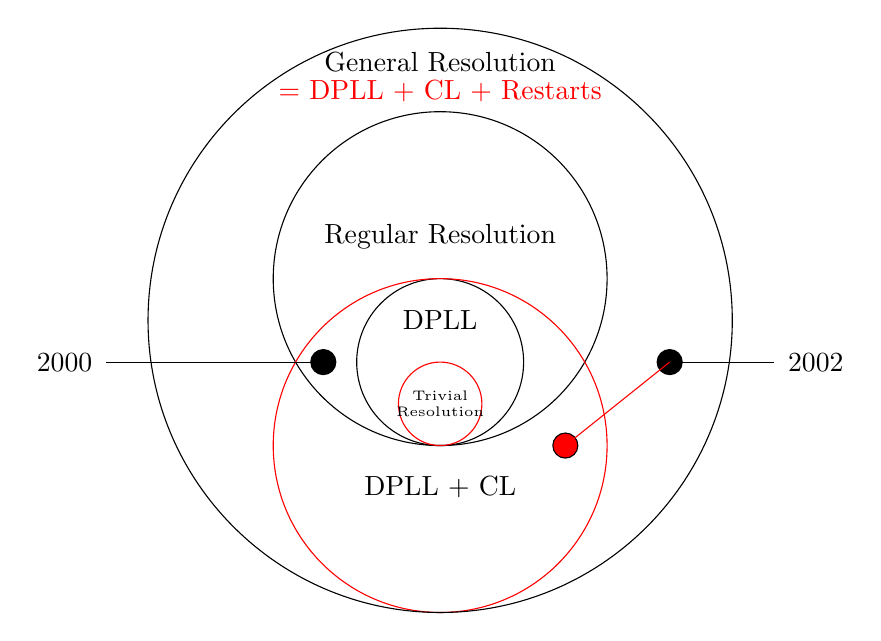
\begin{tikzpicture}[scale=0.53]
      \draw (0,0) circle (2cm);
      \draw (0,2) circle (4cm);
      \draw[color=red] (0,-2) circle (4cm);
      \draw (0,1) circle (7cm);
      \draw[color=red] (0,-1) circle (1cm);
      \node[] at (0,1) {DPLL};
      \node[] at (0,3) {Regular Resolution};
      \node[] at (0,7.2) {General Resolution};
      \node[] at (0,-3) {DPLL + CL};
      \node[] at (0,-0.8) {\tiny Trivial};
      \node[] at (0,-1.2) {\tiny Resolution};
      \node[] at (0,6.5) {\color{red}= DPLL + CL + Restarts};
      \draw[fill=black] (-2.8,0) circle (0.3cm);
      \draw (-8,0) -- (-2.8,0);
      \node[] at (-9,0) {2000};
      \draw[fill=black] (5.5,0) circle (0.3cm);
      \draw (8,0) --  (5.5,0);
      \node[] at (9,0) {2002};
      \draw[fill=red] (3,-2) circle (0.3cm);
      \draw[color=red] (3,-2) --  (5.5,0);
    \end{tikzpicture}
  \end{center}
\end{frame}

\begin{frame}{Learning Schemes}
  \begin{block}{A cut of the conflict graph}
    At each conflict, cutting the conflict graph gives you a clause to learn with equivalent satisfiability.\\
    Here we consider determinist schemes that only use the variables used in the conflict.
  \end{block}
  \vfill
  \begin{block}{Existing schemes}
    \begin{itemize}
    \item Decision clause
    \item \texttt{rel-sat}
    \item 1UIP, 2UIP\dots
    \item \dots
    \end{itemize}
  \end{block}
  
\end{frame}

\begin{frame}{FirstNewCut}
  \begin{exampleblock}{FirstNewCut}
    Non-trivial, non previously known clause closest to the conflict.
  \end{exampleblock}
  \vfill
  \begin{alertblock}{Only used for the proofs}
  \end{alertblock}
  \vfill
  \begin{center}
    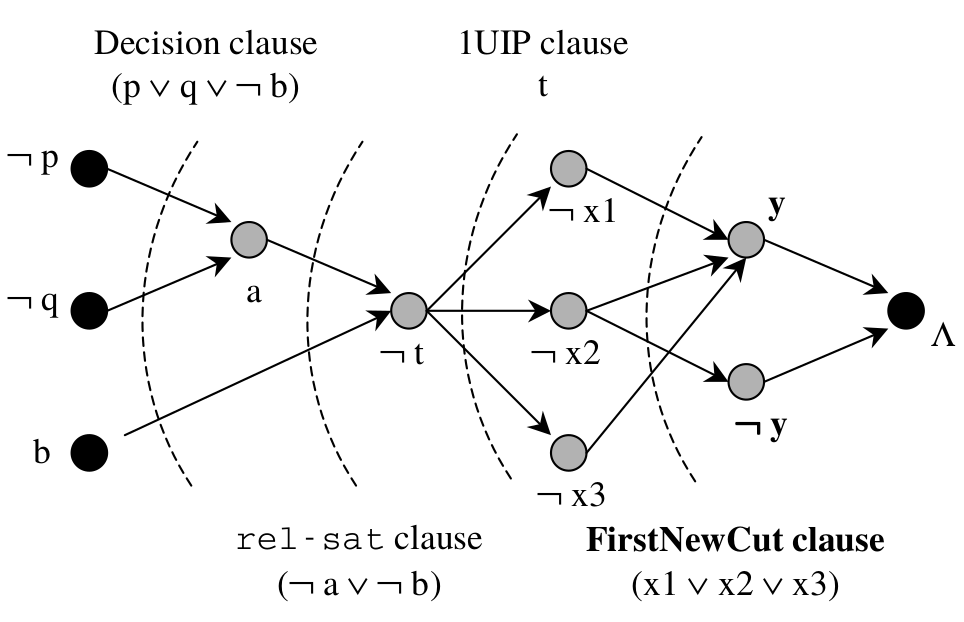
\includegraphics[scale=0.28]{cut.png}
  \end{center}
\end{frame}

\begin{frame}{Clause Learning can be better than Regular}
  \begin{center}
    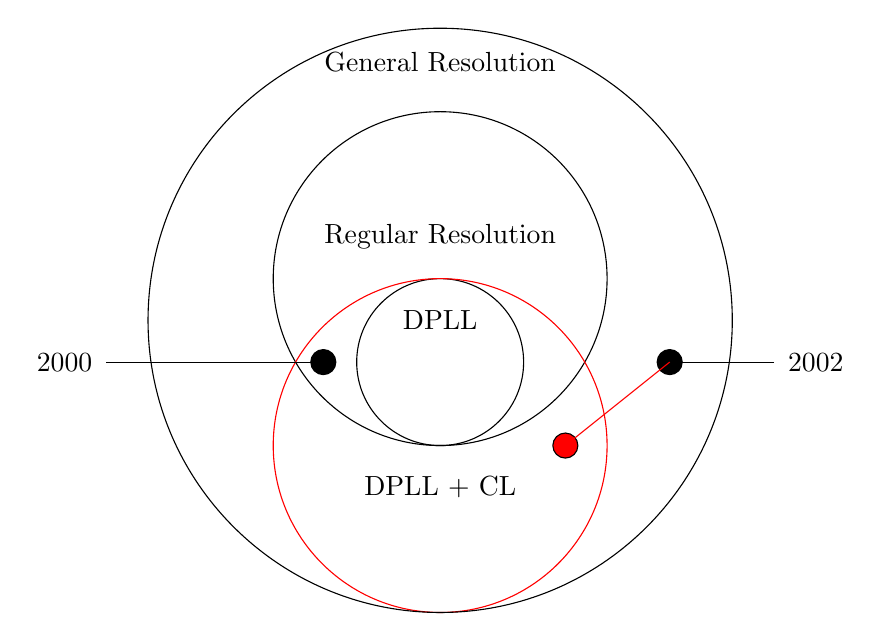
\begin{tikzpicture}[scale=0.53]
      \draw (0,0) circle (2cm);
      \draw (0,2) circle (4cm);
      \draw[color=red] (0,-2) circle (4cm);
      \draw (0,1) circle (7cm);
      \node[] at (0,1) {DPLL};
      \node[] at (0,3) {Regular Resolution};
      \node[] at (0,7.2) {General Resolution};
      \node[] at (0,-3) {DPLL + CL};
      \draw[fill=black] (-2.8,0) circle (0.3cm);
      \draw (-8,0) -- (-2.8,0);
      \node[] at (-9,0) {2000};
      \draw[fill=black] (5.5,0) circle (0.3cm);
      \draw (8,0) --  (5.5,0);
      \node[] at (9,0) {2002};
      \draw[fill=red] (3,-2) circle (0.3cm);
      \draw[color=red] (3,-2) --  (5.5,0);
    \end{tikzpicture}
  \end{center}
\end{frame}


\begin{frame}{Clause Learning can be better than Regular}
  \begin{exampleblock}{Goal}
    Find a family of CNF unsatisfiable formulas, such that it is solved in exponential size by Regular Resolution, but in polynomial size by DPLL + clause learning.
  \end{exampleblock}
  \vfill
  \begin{block}{Method}
    \begin{itemize}
    \item Start with a family of function that separates Regular and General Resolution.
    \item Define a transformation $PT(f,\pi)$ such that solving $PT(f,\pi)$ with DPLL + CL is as long as with General Resolution. But the Regular Resolution is the same size as for $f$.
    \end{itemize}
  \end{block}
      
\end{frame}

\begin{frame}{Clause Learning can be better than Regular - Transformation}
  $f$ unsatisfiable formula with polynomial size General Resolution proof $\pi$ and exponential size Regular Resolution proof.
  \vfill
  \begin{block}{Defining $PT(f,\pi)$}
    All clauses of $f$ and, for each $C\in \pi$, for each $x\in C$, the clause $(\neg x\vee t_C)$ where $t_c$ is a new variable.
  \end{block}
  \vfill
  \begin{alertblock}{Solving with Regular Resolution}
    ``regularity of resolution proofs is preserved under restriction''\\
    Exponential size proof.
  \end{alertblock}
  \vfill
  \begin{exampleblock}{Solving with DPLL+CL}
    Branch on $\neg t_C$ for each $C\in\pi$.\\
    With \textbf{FirstNewCut} you learn $C$. Backtrack on $t_C$.\\
    Polynomial: for each branch on $\neg t_c$ you get one clause of $\pi$.
  \end{exampleblock}
\end{frame}

\begin{frame}{Clause Learning + Restarts equivalent to General Resolution}
  \begin{center}
    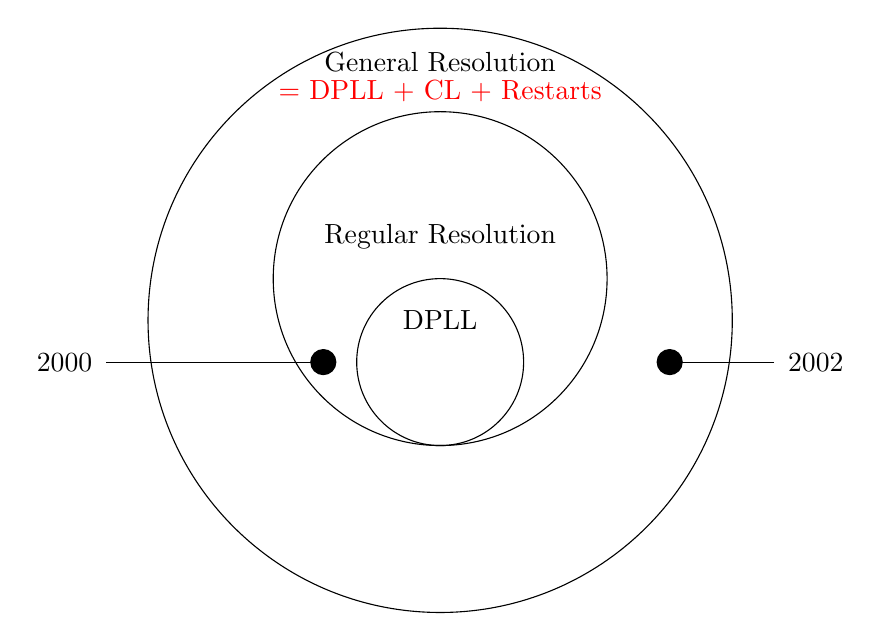
\begin{tikzpicture}[scale=0.53]
      \draw (0,0) circle (2cm);
      \draw (0,2) circle (4cm);
      \draw (0,1) circle (7cm);
      \node[] at (0,1) {DPLL};
      \node[] at (0,3) {Regular Resolution};
      \node[] at (0,7.2) {General Resolution};
      \node[] at (0,6.5) {\color{red}= DPLL + CL + Restarts};
      \draw[fill=black] (-2.8,0) circle (0.3cm);
      \draw (-8,0) -- (-2.8,0);
      \node[] at (-9,0) {2000};
      \draw[fill=black] (5.5,0) circle (0.3cm);
      \draw (8,0) --  (5.5,0);
      \node[] at (9,0) {2002};
    \end{tikzpicture}
  \end{center}
\end{frame}


\begin{frame}{Clause Learning + Restarts equivalent to General Resolution}
  \begin{exampleblock}{Goals: 2 simulations}
    \begin{itemize}
    \item If $f$ has a General polynomial proof, then it also has one with DPLL+CL+restarts.
    \item If $f$ has a DPLL+CL+restarts polynomial proof, then it also has one with General Resolution.
    \end{itemize}
  \end{exampleblock}
  \vfill
  \begin{block}{First Simulation}
    When the resolution proof resolves $(A\vee x) \wedge (B\vee \neg x)$ to get $C$, branch on the negation of the literals of $A$ and $B$.
    You learn $C$ then restart.
  \end{block}

\end{frame}

\begin{frame}{Clause Learning + Restarts equivalent to General Resolution}
  \begin{exampleblock}{Goals: 2 simulations}
    \begin{itemize}
    \item If $f$ has a General polynomial proof, then it also has one with DPLL+CL+restarts.
    \item If $f$ has a DPLL+CL+restarts polynomial proof, then it also has one with General Resolution.
    \end{itemize}
  \end{exampleblock}
  \vfill
  \begin{block}{Second simulation}
    Let $f_n$ with DPLL proof of size $s$.\\
    A previous results shows that in at most $n$ steps we can derive each learned clause with General Resolution.\\
    The resulting proof has size $n\times s$.
  \end{block}
\end{frame}

\begin{frame}{Experimental Results}
  \begin{center}
    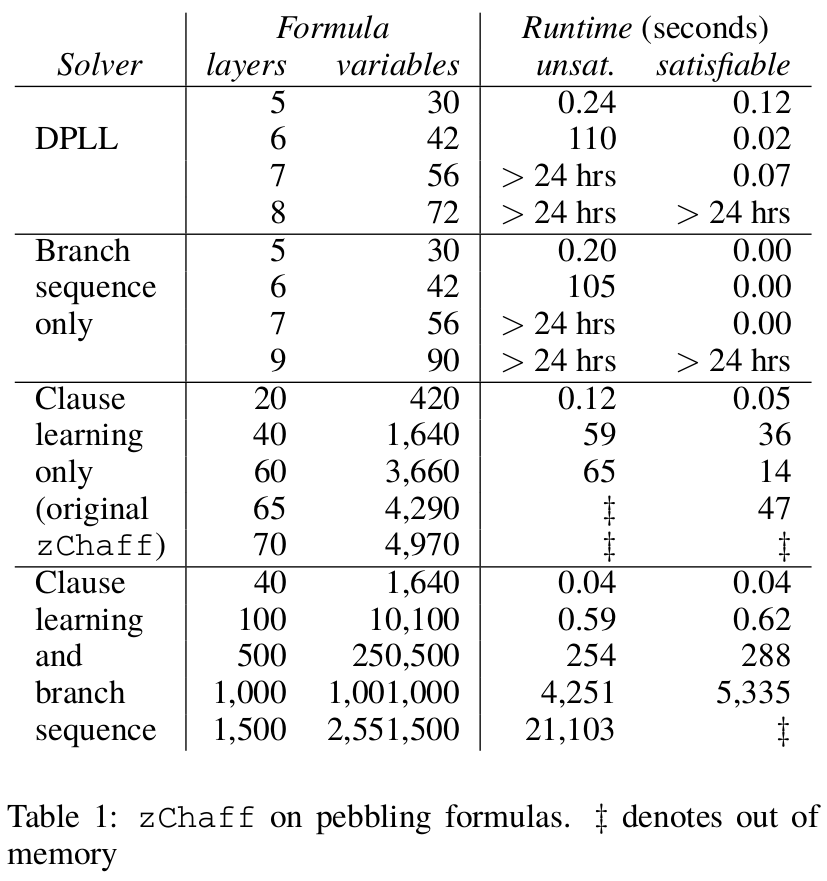
\includegraphics[scale=0.26]{table.png}
  \end{center}
\end{frame}

\begin{frame}{Conclusion}
  \begin{exampleblock}{Clause Learning}
    \begin{itemize}
    \item has potential for small proofs
    \item with restarts, has the same theoretical lower bound as General Resolution
    \end{itemize}
  \end{exampleblock}
  \vfill
  \begin{alertblock}{Good Heuristics are still important!}
  \end{alertblock}
  \vfill
  \begin{block}{Open Problems}
    \begin{itemize}
    \item Which formula for which technique?
    \item Is Regular $\varsubsetneq$ DPLL+CL?
    \end{itemize}
  \end{block}
\end{frame}

\begin{frame}{Overview}
  103 citations in 15 years. The following paper has 286.
  \vfill
  \begin{alertblock}{Questions}
    \begin{itemize}
    \item Experimental Results on transformed pebbling formulas?
    \item Non-deterministic instead of \textbf{FirstNewCut}?
    \item Satisfiable Formulas
    \end{itemize}
  \end{alertblock}
\end{frame}

\begin{frame}{New Results}
  \begin{center}
    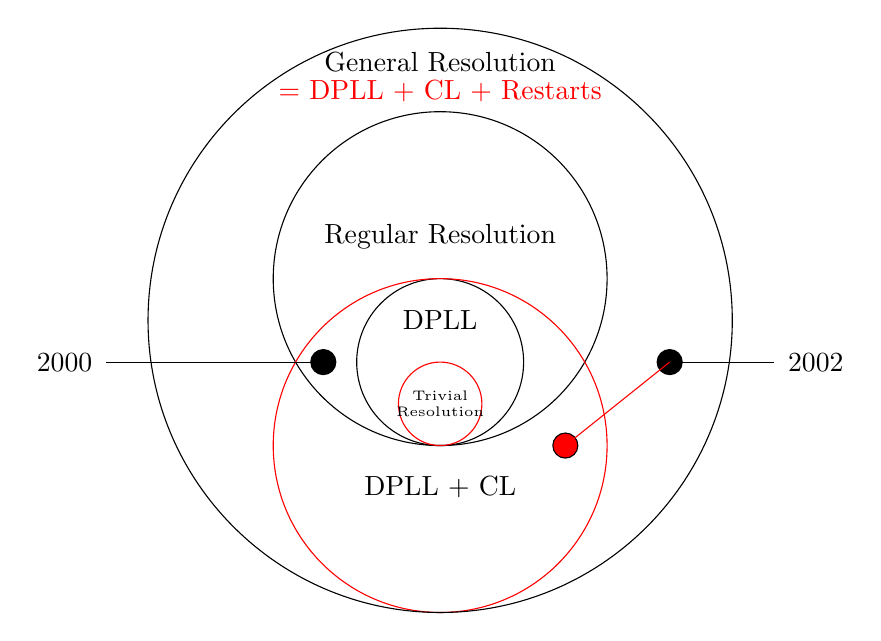
\begin{tikzpicture}[scale=0.53]
      \draw (0,0) circle (2cm);
      \draw (0,2) circle (4cm);
      \draw[color=red] (0,-2) circle (4cm);
      \draw (0,1) circle (7cm);
      \draw[color=red] (0,-1) circle (1cm);
      \node[] at (0,1) {DPLL};
      \node[] at (0,3) {Regular Resolution};
      \node[] at (0,7.2) {General Resolution};
      \node[] at (0,-3) {DPLL + CL};
      \node[] at (0,-0.8) {\tiny Trivial};
      \node[] at (0,-1.2) {\tiny Resolution};
      \node[] at (0,6.5) {\color{red}= DPLL + CL + Restarts};
      \draw[fill=black] (-2.8,0) circle (0.3cm);
      \draw (-8,0) -- (-2.8,0);
      \node[] at (-9,0) {2000};
      \draw[fill=black] (5.5,0) circle (0.3cm);
      \draw (8,0) --  (5.5,0);
      \node[] at (9,0) {2002};
      \draw[fill=red] (3,-2) circle (0.3cm);
      \draw[color=red] (3,-2) --  (5.5,0);
    \end{tikzpicture}
  \end{center}
\end{frame}


\end{document}
